\documentclass[a4paper,10pt]{report}

\usepackage[latin1]{inputenc}
\usepackage[italian]{babel}
\usepackage[pdftex]{graphicx}
\usepackage{float}

\title{Reti neurali e implementazione}
\author{Davide Gessa}
\date{21 Giugno 2010}

\pdfinfo{
  /Title    (Reti neurali e implementazione)
  /Author   (Davide Gessa)
  /Subject  ()
  /Keywords (reti neurali fuzzy statistica matematica machine learning)
}

\begin{document}
\maketitle

\tableofcontents
\setcounter{tocdepth}{4}
\listoffigures

\chapter{Introduzione}
Questa tesi nasce da un vecchio software da me iniziato verso l'inizio del 2009 (e
mai terminato) che riassumeva il frutto di qualche mia curiosita' riguardo 
l'argomento delle reti neurali artificiali; qualche mese fa ho ritrovato i sorgenti 
e mi sono 
interessato nuovamente all'argomento, riscrivendo da zero una nuova liberia (che analizzero' 
in seguito) che implementa alcuni tipi di reti neurali artificiali e alcuni programmi
che utilizzano questa libreria e presentano alcune possibilita' di utilizzo. 
Avevo gia' iniziato una breve trattazione da esporre su un altro mio
progetto, ma ho deciso di iniziare da capo per dedicarmi ad un argomento che
raccoglie in se' piu' materie, come statistica, matematica, informatica e per certe
caratteristiche tecniche anche sistemi.
Per vedere lo sviluppo dei miei progetti "www.inventati.org/dak".

\section{Licenza}
Il proggetto e' rilasciato interamente sotto licenza GPLv2, presente integralmente
nel file "license.txt"; e' riportato qui di 
seguito l'header presente in ogni file sorgente del progetto:
\newline
\newline 
\ttfamily
\textit
    libnnal
    Copyright (C) 2010 Davide Gessa
    
    This program is free software: you can redistribute it and/or modify
    it under the terms of the GNU General Public License as published by
    the Free Software Foundation, either version 2 of the License, or
    (at your option) any later version.

    This program is distributed in the hope that it will be useful,
    but WITHOUT ANY WARRANTY; without even the implied warranty of
    MERCHANTABILITY or FITNESS FOR A PARTICULAR PURPOSE.  See the
    GNU General Public License for more details.

    You should have received a copy of the GNU General Public License
    along with this program.  If not, see <http://www.gnu.org/licenses/>.
\rmfamily
\newline


\section{Strumenti software}
Ecco una lista dei software principali utilizzati per realizzare il progetto e la tesi
che state leggendo; da sottolineare che tutti sono free software e opensource, e che 
lo sviluppo e' avvenuto col sistema operativo linux gentoo ed in parte con freebsd, 
anch'essi free e opensource.
Ecco una lista dei programmi utilizzati:
\begin{description}
\item[gcc] compilatore per il linguaggio C
\item[cmake] sistema di compilazione
\item[vim] editor di testo
\item[subversion] controllo di revisione
\item[gtk+] librerie per interfacce grafiche
\item[gnuplot] programma di plotting matematico
\item[latex] compilatore per il linguaggio \LaTeX
\end{description}



\section{\LaTeX}
Per scrivere la documentazione del sistema e' stato utilizzato il linguaggio di markup
\LaTeX, che permette di preparare dei testi basati su \TeX, un linguaggio di composizione 
tipografica. Utilizzare \LaTeX, permette di risparmiare un tempo notevole per quanto riguarda
la formattazione delle pagine, la creazione degli indici, la visualizzazione di formule matematiche
e molto altro; per questo motivo e' utilizzato da gran parte di accademici, scienziati, matematici
e ingegneri. \LaTeX e' distribuito come software libero ed e' disponibile su molte piattaforme.





\chapter{Reti neurali}
Questo capitolo mira ad esporre il funzionamento di una rete neurale artificiale
e di alcuni algoritmi per l'apprendimento; e' comunque necessario fare una breve
introduzione riguardo il funzionamento delle reti neurali in natura.

\section{Reti neurali biologiche}
Il funzionamento delle reti neurali artificiali, deriva da degli studi effettuati
sulle reti neurali biologiche, presenti, seppur con diverse caratteristiche, 
nel cervello di ogni animale; i primi successi significativi riguardo lo studio 
del funzionamento delle reti neurali sono relativamente recenti, e alcuni aspetti
sono ancora ignoti.
Le reti neurali sono delle strutture costituite da neuroni; 
i neuroni sono classificabili secondo diverse caratteristiche, una di queste
e' la loro funzione:
\begin{itemize}
\item Neuroni sensitivi o neuroni di input: si occupano di ricevere impulsi e stimoli 
		dagli organi sensoriali.
\item Neuroni motori o neuroni di output: generano impulsi di tipo motorio che vengono
		trasmessi agli organi periferici.
\item Interneuroni o neuroni nascosti: elaborano le informazioni fornite dai neuroni 
		sensitivi per trasmetterle ai neuroni motori.
\end{itemize}

Ogni neurone (che sia sensitivo, motorio o un interneurone) e' formato 
principalmente da tre parti:
\begin{itemize}
\item La soma: che comprende il corpo cellulare compreso il nucleo e altri apparati 
		dedicati alla sopravvivenza della cellula.
 
\item Gli assoni: conducono il segnale generato dal soma verso altre cellule neurali.
 
\item I dentriti: son costituiti da diramazioni ad albero che trasportano segnali di 
		altri neuroni, verso la soma; i dentriti hanno la caratteristica di non essere 
		buoni 
		conduttori di segnali nervosi, i segnali ricevuti tendono quindi a diminuire di
		intensita'.
\end{itemize}


\begin{figure}[h]
	\begin{center}	
		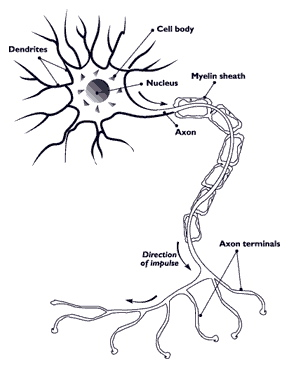
\includegraphics[scale=0.50]{img/neuron.jpg}
		\caption{Struttura di un neurone}
		\label{fig: Struttura di un neurone}
	\end{center}
\end{figure}
 
Gli assoni e i dentriti, comunicano con altre cellule neurali
attraverso dei punti di connessione detti sinapsi. La trasmissione
di un informazione da un neurone all'altro avviene attraverso
l'emissione  di sostanze chimiche dette neuro-trasmettitori 
stimolata da segnali chimici o da segnali elettrici 
generati dal neurone stesso.

Il neurone riceve molti segnali di input tramite i dentriti, 
e rilascia un solo segnale di output tramite l'assone. Il 
segnale di output e quindi il rilascio dei neuro-trasmettitori, avviene
soltanto se la somma dei segnali di input supera una certa soglia;
questa soglia puo' essere ridotta dall'assunzione di
sostanze che provocano eccitazione, (come la caffeina) e puo' essere
aumentata dall'assunzione di tranquillanti.
Le connessioni tra i neuroni non sono immobili, durante la vita le 
connessioni si creano, si trasformano e si distruggono continuamente.

\section{Reti neurali artificiali}
Le reti neurali artificiali sono in sostanza, dei modelli matematici composti
da neuroni artificiali (anche chiamati nodi; sono delle strutture matematiche 
con il compito di emulare in parte il funzionamento di un neurone biologico), 
e dalle loro  interconnessioni che simulano il funzionamento di una rete neurale 
biologica;
le reti neurali artificiali permettono di risolvere problemi (fase di esecuzione)
piu' o meno complessi,
avendo a disposizione dati
non necessariamente esatti, e non utillizzando algoritmi specifici per il problema;
cio' sara' possibile a seguito di un periodo nel quale la rete verra'
istruita a svolgere i compiti desiderati (fase di apprendimento).

\subsection{Neurone artificiale}
Il neurone artificiale e' rappersentato come una struttura matematica, in cui
sono memorizzate determinate informazioni:
\begin{itemize}
\item Stato $ x_i $: lo stato in cui si trova il neurone; ad esempio 
puo' essere 0 o 1 se si tratta
di un neurone binario o da 0 a 1 se si tratta di un neurone a  valori continui.
\item Pesi sinaptici $ \omega_i^k $: sono i valori delle interconnessioni con i neuroni 
dello strato precedente.
\item Errore $ \delta_i $: errore atteso.
\end{itemize}

Per generare l'input netto del neurone bisogna fare la somma del prodotto
dei pesi di ogni connessione dei neuroni dello strato precedente con i loro
valori di output.


\subsection{Tipi di rete}
\subsubsection{Multi Layered Perceptons}
E' il tipo di rete piu' utilizzato; prevede la presenza di neuroni 
divisi in vari strati, generalmente uno di input, uno di output, ed uno
o piu' strati intermedi. Ogni neurone utilizza l'output di tutti i neuroni
dello strato precedente per generare l'output, che sara' utilizzato come
input dallo strato successivo. 

\subsubsection{Self Organization Map}
Le reti dette "a mappa autoorganizzante" prevedono una matrice di neuroni;
per l'apprendimento e' utilizzato un innovativo algoritmo di autoapprendimento,
che aggiorna continuamente i pesi sinaptici utilizzando dei vettori dati
in ingresso, in genere molto grandi. Le uscite sono di solito 2 o 3, ed i 
valori d'uscita nella fase di esecuzione individuano un neurone
della rete, detto vincitore. Le reti som insomma, permettono di assocciare
ad un certo vettore di input, un neurone posizionato nella griglia della rete.


\subsubsection{Hopfield}
Le reti di Hopfield si basano sul concetto delle proprieta' collettive
di un modello costituito da unita' elementari di elaborazione; questo
tipo di rete supera il limite imposto dalle reti mlp che prevedono una sola
direzione per il processo di esecuzione e apprendimento, utilizzando invece
delle reti in cui tutti i neuroni comunicano con tutti gli altri.
Le reti
di Hopfield sono utilizzate specialmente per le memorie assocciative
e per sistemi di ottimizzazione.


\subsection{Apprendimento}
Per poter utilizzare la rete per scopi pratici, bisogna innanzitutto addestrarla
opportunamente per trovare (piu' precisamente imparare) la relazione
tra dati di input e dati di output. L'addestramento puo' essere
eseguito con svariati algoritmi, ma fondamentalmente si
possono distinguere tre grandi tipologie di apprendimento:

\begin{itemize}
\item Supervisionato: consiste nel proporre alla rete dei set di dati di input e i 
corrispettivi
dati di output (risultato degli input); tramite un algoritmo, la rete
impara il legame che c'e' tra essi.
Uno degli algoritmi chiave dell'apprendimento supervisionato, e' l'algoritmo
di propagazione inversa (meglio noto come backpropagation), che mediante
un pattern di input ed uno di output, calcola l'errore per ogni strato
della rete ricalcolando i pesi sinaptici dei singoli neuroni.
L'algoritmo di backpropagation verra' analizzato nei dettagli
nell'articolo dedicato alle reti MLP.


\item Non supervisionato: non prevede nessun intervento esterno, bensi' utilizza
metodi probabilistici per individuare dei possibili input e dei corrispondenti
risultati di output; un esempio famoso e' l'algoritmo di autoapprendimento
utilizzato nelle reti som.


\item Per rinforzo: un algoritmo si occupa di generare azioni e di interpetare il 
risultato della retroazione dell'ambiente stesso, valutando se tale retroazione 
e' positiva o negativa per raggiungere lo scopo prefissato dalla rete.
\end{itemize}



\chapter{Reti MLP e apprendimento supervisionato}
La rete MLP e' il modello di rete neurale artificiale piu' utilizzato; 
prevede la presenza di neuroni artificiali
divisi in vari strati, generalmente uno di input, uno di output, ed uno
o piu' strati intermedi. Ogni neurone utilizza l'output di tutti i neuroni
dello strato precedente per generare l'output, che sara' utilizzato come
input dallo strato successivo. 
In questo capitolo analizzero' in breve gli algoritmi di esecuzione della
rete, e l'algoritmo base di backpropagation per l'apprendimento supervisionato.

\section{Elenco dei simboli}
Ecco una tabella riassuntiva dei simboli che utilizzero' nella schematizzazione
degli algoritmi:
\begin{table}[h]
	\begin{center}
	    \begin{tabular}{  c  c  }
	    $ \delta_i $ & Errore del neurone i \\ 
	    $ \eta $ & Costante di apprendimento \\ 
	    $ \omega_i^k $ & Peso sinaptico del neurone i rispetto al neurone k precedente \\
	    $ x_i $ & Valore del neurone di input i \\ 
	    $ y_i $ & Valore del neurone hidden i \\ 
	    $ z_i $ & Valore del neurone di output i \\ 
	    \end{tabular}
	\end{center}
	\caption{Elenco dei simboli per le reti MLP}
	\label{tab:mlp_symbols}
\end{table}


\section{Esecuzione}
La fase di esecuzione consiste nel fornire alla rete dei dati di input,
elaborarli ed ottenere dei dati di output; l'esecuzione della rete
consiste in 3 step:

\begin{itemize}
\item Inserimento i dati di input nei neuroni di input.

\item Per ogni neurone di ogni strato nascosto e dello strato di output, 
calcolo dello stato del neurone tramite la formula:

\[
	y_i = f(\sum (\omega_i^k * x_k))
\]

\item Prelevamento degli output dai neuroni di output.
\end{itemize}

\section{Back Propagation}
Il "back propagation" (propagazione inversa) e' l'algoritmo piu' diffuso
per l'addestramento delle reti neurali di tipo MLP; l'algoritmo puo' essere
riassunto in 2 step:

\begin{itemize}
\item Si inseriscono i valori di input del pattern di addestramento nei neuroni 
dello strato di input. Si esegue la rete, e si calcola l'errore delta di output:
per ogni neurone dello strato di output si calcola la differenza tra il valore 
desiderato ( $ d_i $ ) e quello ottenuto dall'esecuzione, poi il valore ottenuto
viene moltiplicato per la derivata
della funzione di trasferimento avente come argomento il valore di
output ottenuto dalla rete nello stato in cui e' il neurone attualmente:

\[
 \delta_i = (d_i - z_i) * f'(z_i)
\]

Successivamente si calcola l'errore delta di ognuno degli strati nascosti
della rete sino ad arrivare al primo neurone nascosto:

\[
 \delta_i = (\sum (\delta_k * \omega_k^i)) * f'(y_i))
\]



\item I valori cosi' ottenuti permetteranno di modificare i pesi delle connessioni
di ogni strato per ogni neurone, 
per ottenere un valore di output piu' verosimile al valore desiderato
Per ogni neurone di output e di hidden quindi:

\[
 \omega_i^k = (\sum (\eta * y_k * \delta_i))
\]

\end{itemize}

Il procedimento termina qui; si passa ad un altro pattern di addestramento
e si riprende dal punto uno.

%	// Aggiorna i pesi dello strato hidden
%	for(j = 0; j < n->hidden_n; j++)
%	{
%		for(k = 0; k < n->input_n; k++)
%			(n->hidden[j]).weights[k] += n->learning_rate * (n->hidden[j]).delta * (n->input[k]).value;
%		(n->hidden[j]).bias += n->learning_rate * (n->hidden[j]).delta;
%	}



%da qui in poi e' okkey

\section{Pattern Recognition mediante rete neurali}
Il pattern recognition (riconoscimento di pattern, in italiano), 
e' una delle possibili applicazioni delle reti neurali; 
il pattern recognition in se', e' un processo di 
riconoscimento e classificazione di pattern, partendo
da un insieme di dati grezzi in input. Per l'addestramento vengono
generati vari pattern per ogni carattere (se i pattern sono caratteri); 
questi pattern vengono
passati alla rete neurale come dati di input, e come output viene 
specificato di che carattere si tratta; successivamente si esegue 
l'algoritmo di backpropagation per un cospicuo numero di epoche;
la rete cosi' addestrata sara' in grado di riconoscere anche pattern diversi
da quelli utilizzati per l'addestramento.




\chapter{Neural Network Abstraction Layer}
La mia liberia prende il nome di "nnal", ovvero "neural network abstraction layer" 
(layer
di astrazione di reti neurali); il motivo di questo nome deriva dal fatto che lo scopo 
e' quello
di realizzare un framework che offre strumenti semplici per simulare reti neurali, 
risparmiando ai
programmatori l'arduo compito di crearsi una libreria. Nnal mira a studiare nei 
dettagli
problematiche relative al calcolo e alla memoria utilizzata, ottimizzando al meglio 
il codice e prevedendo
l'utilizzo di cuda e opencl per il calcolo tramite gpu;
attualmente i tipi di rete implementati sono due:
\begin{itemize}
\item Reti MLP, implementate completamente
\item Reti SOM, ancora in fase di sviluppo
\end{itemize}

\section{Simulare una rete MLP}
La libreria nnal offre semplici funzioni per simulare le reti MLP e 
per eseguire l'apprendimento tramite backpropagation; supponiamo di voler
creare una rete per svolgere la funzione logica or;
per prima cosa decidiamo il numero di neuroni per ogni layer, in
questo esempio 2 neuroni per l'input
3 per l'hidden e 1 per l'output:

\begin{verbatim}
int layers[] = { 2, 3 1 };
\end{verbatim}


Si crea poi una rete neurale con 3 layer passando l'array precedentemente creato:

\begin{verbatim}
mlp_neural_network_t *n = mlp_new(layers, 3);
\end{verbatim}


Decidiamo poi che funzioni matematiche vogliamo utilizzare per il trasferimento dei dati
da un neurone all'altro (nella libreria sono gia' implementate alcune funzioni di 
trasferimento);
ad esempio utilizziamo la sigmoide logistica in modo che ci sia possibile verificare 
l'approssimazione dei risultati:

\begin{verbatim}
n->transf_func = &sigmodial;
n->transf_func_derivate = &sigmodial_derivate;
\end{verbatim}


Ora facciamo un semplice esempio di addestramento; l'unico algoritmo di addestramento 
implementato
per le reti mlp e' l'algoritmo di backpropagation. Utilizziamo un ciclo for per far 
elaborare alla rete
i pattern di addestramento da noi generati, per un certo numero di epoche; il numero 
delle epoche ed il 
numero di pattern devono essere adeguati in modo da garantire un errore delta 
trascurabile.
I pattern di addestramento sono fondamentalmente due array, il primo, contente i dati 
di input
ed il secondo contenente i dati di output:
 
\begin{verbatim}
for(i = 0; i < N_EPOCHE; i++)
{
	in[0] = 1.0;
	in[1] = 1.0;
	out[0] = 0.0;	
	mlp_back_propagate(n, in, out);

	in[0] = 1.0;
	in[1] = 0.0;
	out[0] = 1.0;	
	mlp_back_propagate(n, in, out);

	in[0] = 0.0;
	in[1] = 1.0;
	out[0] = 1.0;	
	mlp_back_propagate(n, in, out);

	in[0] = 0.0;
	in[1] = 0.0;
	out[0] = 0.0;	
	mlp_back_propagate(n, in, out);

	printf("epoch: %d\n",i);
}
\end{verbatim}


Sono inoltre presenti delle funzioni per salvare la rete in un file e per
caricare una rete da file:

\begin{verbatim}
mlp_save(n, "saved/or.nn");

n = mlp_load("saved/or.nn");
\end{verbatim}


Successivamente all'addestramento, e' possibile utilizzare la rete; facciamo un test
passando la combinazione 0, 1 in input; il risultato verra' messo dalla funzione
nell'array out e dovrebbe essere 1:

\begin{verbatim}
in[0] = 0.0;
in[1] = 1.0;
mlp_execute(n, in, out);
\end{verbatim}

\newpage
\section{Visualizzazione reti con GtkWidget}
Libnnal implementa anche un widget per gtk+ che permette di visualizzare
una rete neurale graficamente, quindi i neuroni di ogni layer, le relative connessioni
tra di essi ed i pesi sinaptici delle connessioni. I diversi valori delle connessioni
e dei neuroni sono rappresentati tramite l'utilizzo di colori diversi.

L'integrazione
in un applicazione gtk e' molto semplice; per la creazione e l'utilizzo
della rete si fa riferimento al codice visto in precedenza, mentre le funzioni
per utilizzare il widget sono principalmente due:
\begin{itemize}
\item La prima crea il widget:
\begin{verbatim}
GtkWidget *mlp = gtk_mlp_new();
\end{verbatim}

\item La seconda assegna la rete neurale al widget (viene utilizzato un puntatore,
quindi si puo' operare sulla rete "net", ottenendo le modifiche anche sul widget:
\begin{verbatim}
gtk_mlp_set_network(GTK_MLP(mlp), net);
\end{verbatim}
\end{itemize}


\section{Applicazioni software}
Ho realizzato svariati programmi programmi in C, alcuni con un interfaccia
grafica in gtk+, per mostrare varie applicazioni della libreria di astrazione:
\begin{itemize}
\item bptimetest: test sui tempi di apprendimento
\item epochtest: test sul variare del numero di epoche di apprendimento
\item gtkmlp: utilizzo di reti mlp con un interfaccia gtk
\item gtkmlptest: test del widget mlp per gtk
\item mlptest: vari esempi di utilizzo delle reti mlp
\item patterngtk: riconoscimento di pattern con interfaccia gtk
\item patterntest: test di pattern recognition
\end{itemize}

Di questa lista pero', ne analizzero' in specifico solo alcuni.

\newpage
\subsection{Neural network}
MlpGtk permette di creare una rete neurale generica, decidendo
il numero di neuroni per ogni layer, il coefficiente di apprendimento
ed il tipo di funzione di trasferimento; dopo la creazione della rete
e' possibile:

\begin{itemize}
\item Addestrare la rete tramite dati prelevati da file
\item Osservare il cambiamento dei pesi sinaptici graficamente durante 
e dopo l'addestramento
\item Impostare dei valori ai neuroni di input per farli elaborare alla rete
\item Salvare e caricare la rete
\end{itemize}

Ecco uno screenshoot della schermata principale:
\begin{figure}[!ht]
	\begin{center}	
		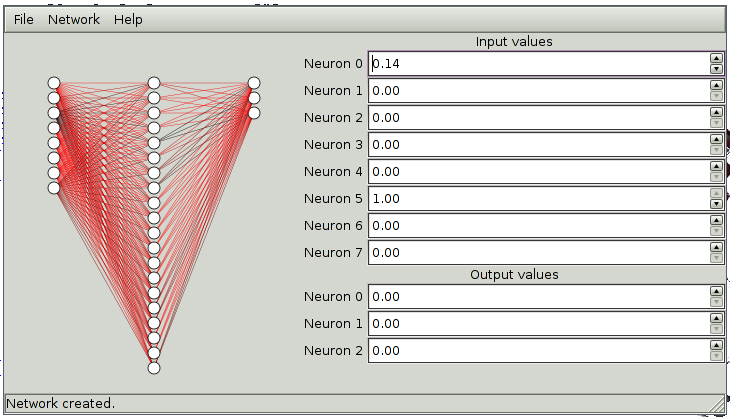
\includegraphics[scale=0.6]{img/screen/neuralnet1.png}
		\caption{Neural Network in GTK+}
		\label{fig: Neural Network in GTK+}
	\end{center}
\end{figure}


\newpage
\subsection{Pattern Recognition}
PatternGtk invece,  e' un programma per il riconoscimento
di pattern, fondamentalmente di lettere e numeri; con qualche
piccola modifica e' possibile utilizzarlo anche per altri tipi di dati.
Il programma permette di indicare una cartella contenente file png
(per ora solo 64x64 in scala di grigi), selezionare il numero di epoche, 
e avviare il processo di apprendimento; e' possibile poi utilizzare un'altra 
immagine, con le stesse caratteristiche dei pattern di addestramento, 
per testare la rete ed ottenere in output il codicce ascii della lettera 
corrispondente all'immagine. 

Per fare test diversi, ho creato vari set di pattern, in figura possiamo
vedere un test con le lettere cirilliche (translitterate in lettere latine):

\begin{figure}[!ht]
	\begin{center}	
		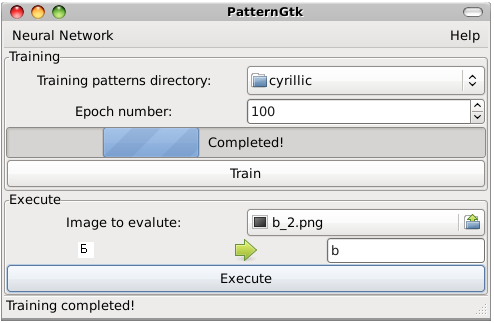
\includegraphics[scale=0.5]{img/screen/patrec1.png}
		\caption{Pattern Recognition in GTK+ - Alfabeto Cirillico}
		\label{fig: Programma di Pattern Recognition in GTK+ - Cirillico}
	\end{center}
\end{figure}


E qui un esempio con l'alfabeto italiano:
\begin{figure}[!ht]
	\begin{center}	
		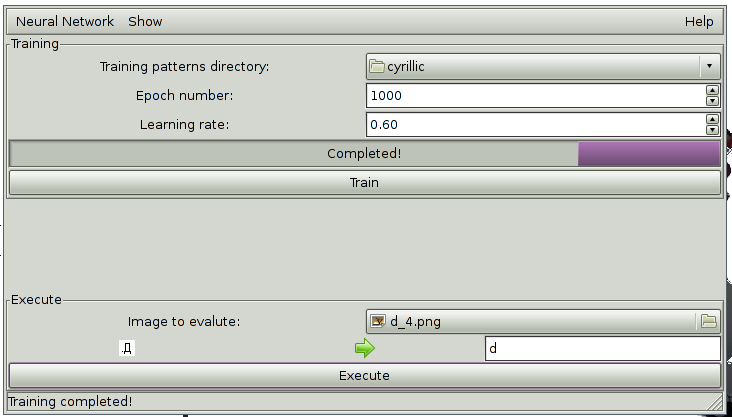
\includegraphics[scale=0.5]{img/screen/patrec2.png}
		\caption{Pattern Recognition in GTK+ - Alfabeto italiano}
		\label{fig: Programma di Pattern Recognition in GTK+ - Italiano}
	\end{center}
\end{figure}


\newpage
Ho realizzato inoltre dei test sull'andamento dell'errore delta calcolato su
un set di pattern di 22 caratteri per differenti numeri di epoche. Come si
puo' notare, si raggiunge un valore di errore di circa 0.3 dopo circa 1000 epoche;
aumentando il numero di epoche si ottiene un andamento asintotico sopra questo valore:

\begin{figure}[!ht]
	\begin{center}	
		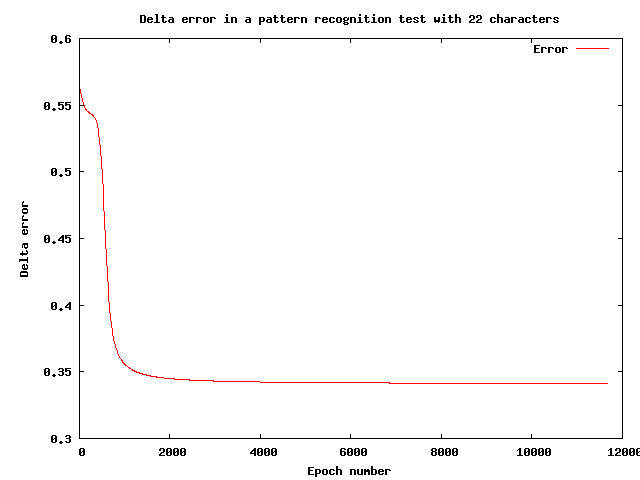
\includegraphics[scale=0.5]{img/stat/epoch_pattern.png}
		\caption{Pattern Recognition - Epoch test}
		\label{fig: Pattern Recognition - Test delle epoche}
	\end{center}
\end{figure}



\newpage
\subsection{Mlp Widget}
In figura possiamo vedere l'utilizzo del widget gtk nel programma
per il pattern recognition:

\begin{figure}[!ht]
	\begin{center}	
		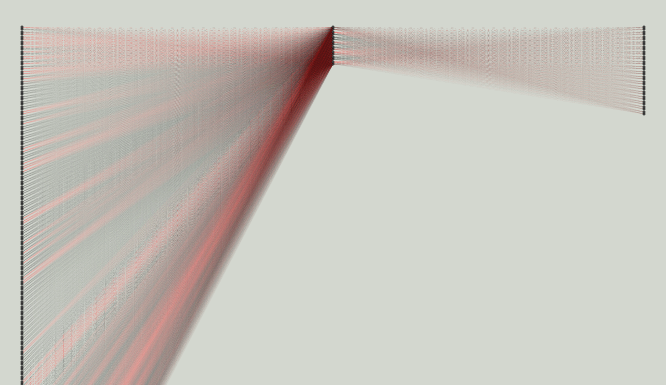
\includegraphics[scale=0.5]{img/screen/cairoshow.png}
		\caption{Pattern Recognition in GTK+ - Visualizzazione grafica}
		\label{fig: Programma di Pattern Recognition in GTK+ - Visualizzazione}
	\end{center}
\end{figure}


Ed un esempio di rete piu' piccola creata con MlpGtk:

\begin{figure}[!ht]
	\begin{center}	
		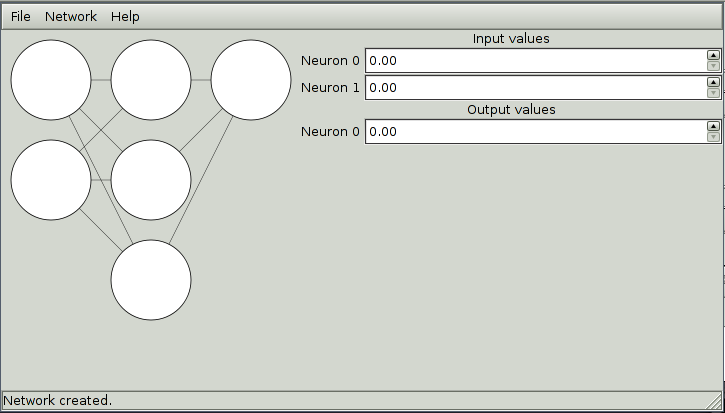
\includegraphics[scale=0.65]{img/screen/mlp_gtk.png}
		\caption{Reti MLP in GTK+ - Visualizzazione grafica}
		\label{fig: Reti MLP in GTK+ - Visualizzazione}
	\end{center}
\end{figure}

\chapter{Bibliografia}
\begin{thebibliography}{Bibliografia}
	\bibitem{lamport-latex2} Silvio Cammarata - Reti neurali, dal Percepton alle reti caotiche e neuro-fuzzy
	\bibitem{lamport-latex2} Christopher M. Bishop - Pattern Recognition and Machine Learning
\end{thebibliography}

\appendix


\end{document}

